\documentclass{article}

\usepackage{graphicx}
\usepackage{natbib}
\usepackage[margin=1in]{geometry}
\usepackage{hyperref}
\usepackage{listings}
\usepackage{caption}
\usepackage{subcaption}

\let\cite\citep
\title{A parallel-in-time solver for the heat equation}
\author{Noah Brenowitz and Irena Vankova}
\date{May 18, 2015}
\begin{document}
\maketitle
\section{Introduction}
\label{sec:intro}

The aim of this project is to test the ``Parallel-in-time'' concept
on the heat equation 
\[ u_t = \Delta u \]
with periodic boundary conditions. 
The parallel-in-time strategy is distinct from any sort of spatial
domain decomposition approaches, and we do not implement any spatial
parallelism in this example. 
We choose a parallel in time strategy based on \cite{falgout2014parallel}. We solve the equation on two temporal grids, coarse and fine, where the solutions on the fine grid provide initial data for the the next coarse time step. Details are described in Section~\ref{sec:code}.

\section{Heat equation solver}
\label{sec:ehat}

The serial implementation of the heat equation solver is relatively
straightforward. The typical 2 dimensional discrete laplacian is used
with a implicit trapezoid rule time stepping procedure
(e.g. Crank-Nicolson). The advantage of the Crank-Nicolson scheme is
that it is unconditionally stable like the backward Euler scheme, but
also has second order accuracy.

The solver requires a uniform grid in both
spatial dimensions. In detail, if the discrete laplacian operator is
given by
\[ (L u)_{i,j} = u_{i-1,j} + u_{i+1,j} + u_{i,j-1} + u_{i, j-1} - 4 u_{i,j}, \]
the time step is $\tau$ and the spatial grid size is $h$. Then the
implicit trapezoid rule gives
\[ u^{n+1}  = \frac{\lambda}{2} \left( Lu^n + Lu^{n+1} \right),\]
where the CFL number $\lambda = \tau / h^{2}$.

In practice, this iteration can be written as a matrix
multiplication followed by a linear solve in the following way
\begin{equation}
  \label{eq:time-step}
  u^{n+1} = \left( I- \frac{\lambda}{2} L \right)^{-1} \left(I+\frac{\lambda}{2}L \right) u^n.
\end{equation}


\section{Code design}
\label{sec:code}

The code for this final project is available at \url{https://github.com/nbren12/hpc15final}.
It consists of two parts:
\begin{itemize}
\item The serial heat equation solver provides a library in
  \verb|./src/| called \verb|liblaplace.a| with a simple function that
  evolves the heat equation forward in time with a given time
  step. The signature of this function is
\begin{lstlisting}
void evolve_heat_equation_2d(double *x, int n, double dx,
			     int nt, double dt, int output_interval);
\end{lstlisting}
  
This header provides C-linkage, but the library is written in C++
using a MATLAB like linear algebra package called
\href{http://arma.sourceforge.net/}{Armadillo++} for the sparse linear
solve and matrix multiplications. Armadillo++ is essentially a
high-level wrapper for libraries like BLAS, SuperLU, and LAPACK. The
advantage over using MATLAB or numpy is that there is no temporary
arrays formed with expressions like \verb|a = b + c|.

\item To test the parallel in time idea, we fix special grid and the final time $T$ and choose total number of time steps $nt$. The fine grid time step is $dt = T/nt$. We compute solution on this fine grid by calling evolve\_heat\_equation\_2d and this fulfills the purposed of exact solution $u_{exact}$ for the comparison of time parallel tests. Next we choose a coarse time step $dt_c$, and number of coarse time steps $nt_c$ will equal the number of processors used, $np$. We evolve the equation on the coarse time grid, and we take the coarse grid values as initial values to be evolved independently on a fine grid of length $nt/nt_c$ on each of the $np$ processors. This process is repeated maximum of $np$ times and in each iteration one less processor is used. After each iteration we compute the relative error $E = \sqrt{\frac{\sum{(u_{exact} - u)^2}}{\sum{(u_{exact} )^2}}}$ and we set a tolerance of 10\%, to stop iterating when $E<0.1$. There are time savings when the number of iterations is smaller than number of iterations required converge exactly to the fine grid solution ($np$).

\end{itemize}

\section{Scalability}
\label{sec:scale}

We ran tests with 640,1280, 2560, 5120 and 10240 total time steps ($nt$) and for 5, 10, 20, 40 and 80 time steps per processor. This together gave us 25 cases to compare. The measure of savings in time we use is the ratio of required iterations to get within the tolerance to $np$, (percentage of time saved). The results are summarized in Figure~\ref{fig:scal} . On the top graph each color represents fixed amount of time steps per processor (coarse block). As we refine the time step ( = increase the number of coarse blocks), the utility of parallelization in time improves. Due to the simplicity of heat equation, at some point the refined solution is as good as the coarse solution (that is what 100\% time saved means). On the lower graph each color represents fixed $nt$. Given that, parallelizing with a higher number of coarse blocks improves the performance in time.
Figure~\ref{fig:conv} shows that the convergence to the solution on the corresponding fine grid is exponential, for some sample runs.


\begin{figure}
      \begin{center}
	      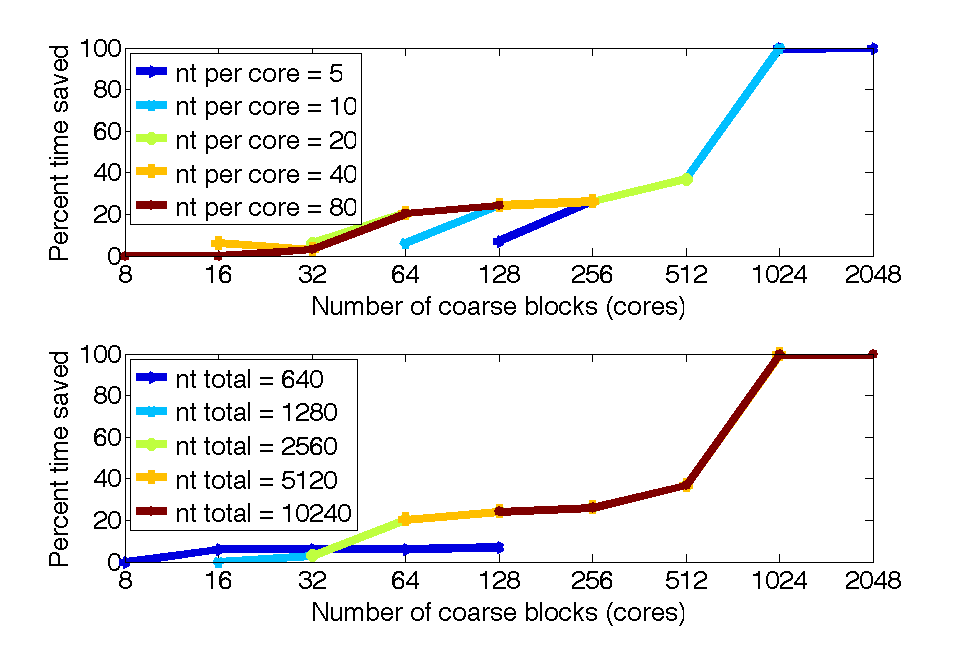
\includegraphics[width=16cm]{scalability_test}
      \end{center}
\caption{}
\label{fig:scal}
\end{figure}  

\begin{figure}
      \begin{center}
	      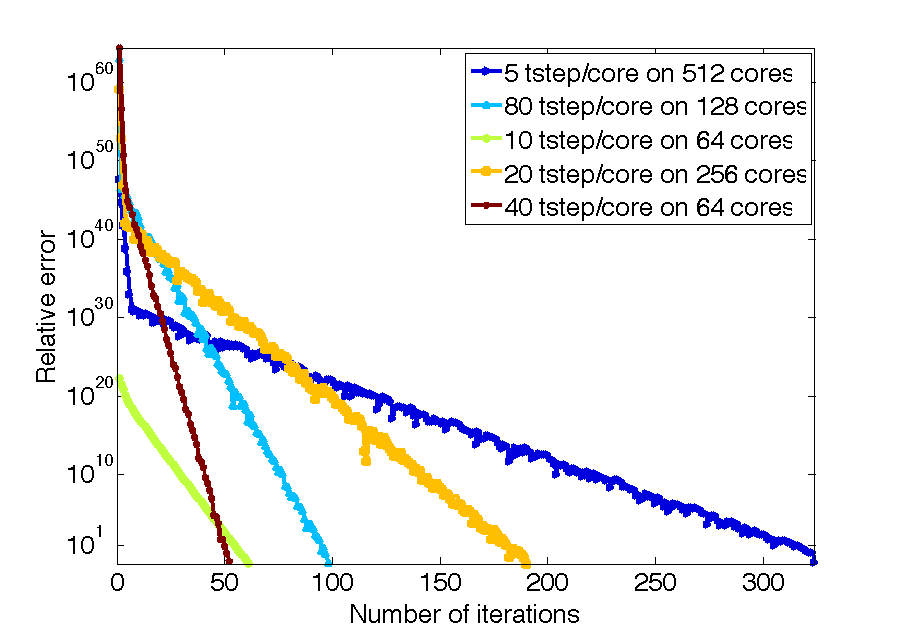
\includegraphics[width=16cm]{convergence}
      \end{center}
\caption{}
\label{fig:conv}
\end{figure}  


\section{Conclusion}
\label{sec:concl}

Once an algorithm is perfectly spatially parallelized, it may be possible, based on the system of equations, to speed up the computation by parallelizing in time. We tested this idea on heat equation in two dimensions, and obtained good results, which we attribute mainly due to the simplicity of the equation. Although an interesting idea, we found this approach rather wasteful, due to the amount of processors needed for repetitive iterative calculations, in order to achieve significant time savings. This conclusion however maybe a result of personal philosophy rather than anything else.




% Bibliography
\bibliographystyle{authordate1}
\bibliography{refs}
\end{document}
